% main.tex, to be used with thesis.tex
% This contains the main work of your thesis.

%\bibliography{thesis}  % uses the references stored in Chapter1Radar.bib

\chapter{Proposal of a Data Persistence in Sensor Networks Taxonomy}
\label{chap:taxonomies}

As reveled in the previous chapter, data persistence for sensor
networks require an understanding of not only the properties of the
infrastructure of a given sensor network, but also of the properties and nature
of the collected data themselves. In order to
identify these concepts more clearly, each section of this chapter proposes an
individual taxonomy based on the aspects described in the literature
review. Then, it briefly discusses the relationships among them.

The root of word ``Taxonomy'' is the Greek taxis, meaning 'order' or
'arrangement', and, nomos in Latin, meaning 'law' or 'science'). In
short, taxonomy is defined as the practice and science of classification and
uses the taxonomic units of ``taxa'', the plural form of ``taxon''
\cite{taxonomy}. Similarly, hierarchical diagram is used to relate each of the
taxa to their main taxon. 

\section{Purpose of the Sensor Data Taxonomy}

As delineated in Section \ref{sec:sn-data-purpose}, the purpose of the
collected data from sensor devices determines how the collected data is
retrieved and used in the network. In such a fashion, this taxonomy relates to
how the collected data is used, and should be the primary question answered 
during the analysis of a sensor network. The taxa related to this
taxonomy, depicted in Figure \ref{fig:taxonomy-data-purpose}, is described as
follows:

\begin{figure}[h]
  \centering
  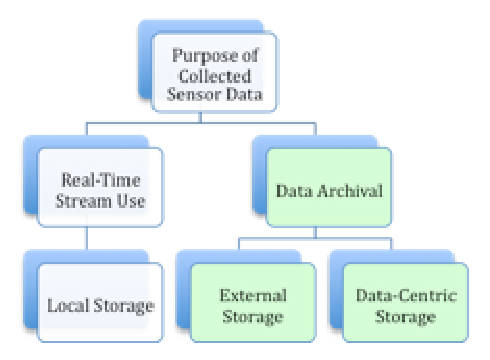
\includegraphics{../diagrams/taxonomy-data-purpose}
  \caption{The Purpose of Sensor Data Taxonomy}
  \label{fig:taxonomy-data-purpose}
\end{figure}

\begin{itemize}
  \item \textbf{Real-time Data Stream}: the collected data is accessed
  on-the-fly from the sensor device as a real-time data stream, and may have a
  short life cycle as it temporarily resides in memory;
  \item \textbf{Data Archival}: the collected data is used for historical
  purposes and is related to the historical data analysis \cite{sn-intro01,
  sn-intro02} or Information Fusion \cite{sn-info-fusion}. 
\end{itemize}

\section{Location of the Sensor Data Taxonomy}

The location where the collected data is stored plays an important role
in the different aspects of the access to the collected data from sensor
devices, as shown in Section \ref{sec:sn-storage-locations}. Figure 
\ref{fig:taxonomy-data-location} depicts this taxonomy, which can be
described as follows:

\begin{figure}[h]
  \centering
  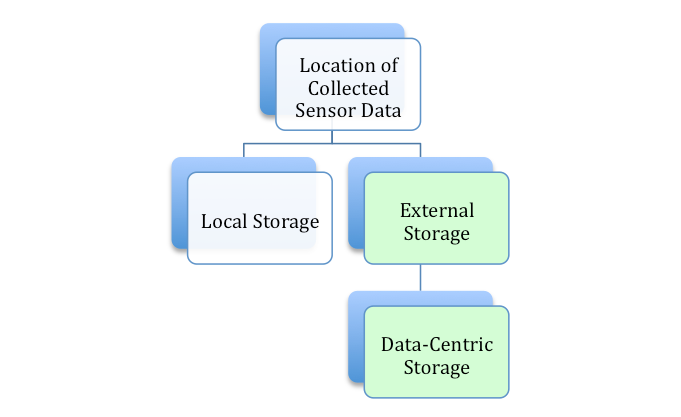
\includegraphics{../diagrams/taxonomy-data-location}
  \caption{The Location of Sensor Data Taxonomy}
  \label{fig:taxonomy-data-location}
\end{figure}

\begin{itemize}
  \item \textbf{Local Storage}: characterizes the place the collected data is
  temporarily located in-memory, or in a secondary storage device on a node
  located in-network;
  \item \textbf{External Storage}: The collected data is usually located in an
  external storage device with a data management system such as a relational
  database. When the collected data occupies different external storage devices, the
  strategy is called \textbf{Data-Centric Storage}
  \cite{sn-data-centric-storage}, being organized by categories based on the
  collected data keys and values. In other words, what characterizes this
  taxon is the presence of a data partitioning strategy to store the collected
  data.
\end{itemize}

\section{Data Model Taxonomy}

One of the fundamental challenges in the development of a persistence storage
in sensor networks is related to the data model chosen to represent the
collected data. This taxonomy relates to the data model used to design the 
collected data, as shown in Figure \ref{fig:taxonomy-data-model}, and is 
described as follows.

\begin{figure}[h]
  \centering
  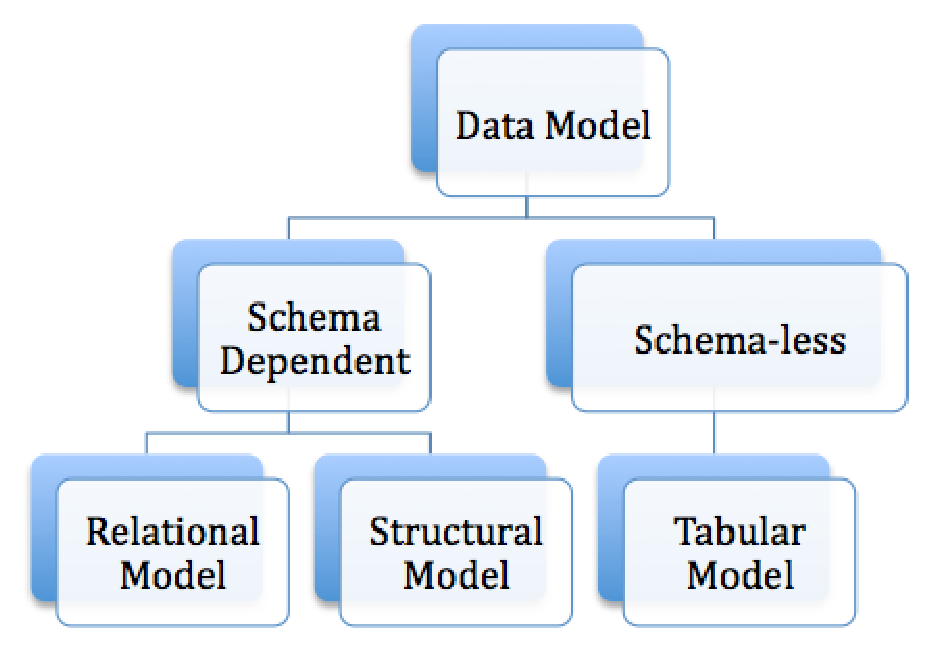
\includegraphics[scale=0.5]{../diagrams/taxonomy-data-model}
  \caption{The Data Model Taxonomy}
  \label{fig:taxonomy-data-model}
\end{figure}

\begin{itemize}
  \item \textbf{Schema-Dependent Models}: this data model requires the
  definition of a master schema that describes the data through a rigorous
  data modeling process prior to the insertion of the data. Examples of this
  model is the traditional Relational Data Model\cite{relational-model}, as
 well as the Structured Data Models such as the XML \cite{xml};
  \item \textbf{Schema-less Models}: contrary to the former taxon, schema-less
  data models do not require the definition of a data schema or table
  definition. Instances of such a data model is the use of the 
  Tabular Data model.
\end{itemize}

\section{Data Description Taxonomy}

Particularly related to how the collected data is described, different projects
provide data persistence describing the collected data by using its natural
properties, or associating textual descriptions or keywords for the data. The
way to describe or label data can follow different guidelines such as data provenance
and annotations, discussed in Section \ref{sec:sn-data-description}. The description of the
properties should take into account the different values of the nature of the
data and any other description needed. Therefore, the taxa that compose the
Data Description taxonomy, shown in Figure
\ref{fig:taxonomy-data-description}, are described as follows:

\begin{figure}[h]
  \centering
  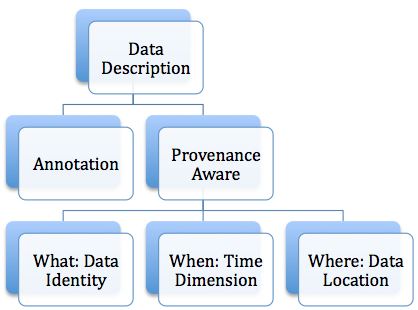
\includegraphics[scale=0.5]{../diagrams/taxonomy-data-description}
  \caption{The Data Description Taxonomy}
  \label{fig:taxonomy-data-description}
\end{figure}

\begin{itemize}
  \item \textbf{Provenance-Aware}: when the collected data is categorized based
  on the nature of the data, \textbf{What: Data Identity} is the data type
  that uniquely identifies the collected data from sensors. Similarly, the
  \textbf{When: Time Dimension}, is related to instances of time relative to the
  collected data: \textbf{valid} and \textbf{transaction} times. The former is
  used to identify when the data was collected, whereas the latter when the data was
  transmitted to the data sink where the query processing acts. Finally, the
  \textbf{Where: Data Location} identifies the point where the collected data
  was observed by the sensor device. Usually the latitude and longitude as the
  GPS coordinates;
  \item \textbf{Annotations}: the annotation of the collected data, through the
  use of keywords, full-text description, or any other method that helps
  describe the collected data. It is important to note that this type of data
  does not makeup part of the collected data from sensors. Rather, they
  complement the observations of what was perceived by the sensor devices.
\end{itemize}

\section{Query Processing Mechanism Taxonomy}

The query processing mechanism in sensor networks is directly related to how
and where the collected data is used and stored, as shown in Section
\ref{sec:query-process}. The following taxa are related to the
different types of query processing mechanisms and summarized in Figure
\ref{fig:taxonomy-query-mechanism}:

\begin{figure}[h]
  \centering
  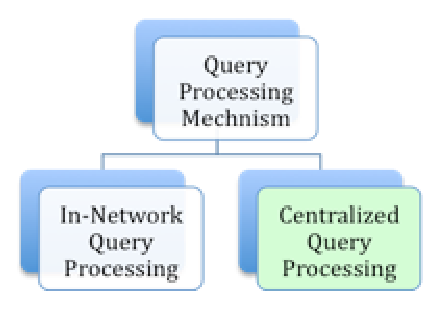
\includegraphics{../diagrams/taxonomy-query-mechanism}
  \caption{The Query Processing Mechanism Taxonomy}
  \label{fig:taxonomy-query-mechanism}
\end{figure}

\begin{itemize}
  \item \textbf{In-Network Query Processing}: when the data node is the
  sensor device itself, and it uses the local storage mechanism, then the
  sensor node is able to reply to the request related to the observations of the 
  environment defined by the sensor device. In this way, the query takes 
  place in the network itself, and usually returns values related to the current
  state of the environment;
  \item \textbf{Centralized Query Processing}: as developed by a single 
  relational database server, the data queried from a centralized data
  network sink in order to be reused. In general, this approach is used when
  the purpose of data is archival data.
\end{itemize}

\section{Data Volume Taxonomy}

When it comes to the data volume produced during a time frame, different ranges
are reported from different types of sensor networks. Depending on the types
of data produced such as numerical or images, they can be in the orders of
Megabytes (1MB = 1000KB = ~10\superscript{3} bytes), Gigabytes (1GB =
1000\superscript{3} = 10\superscript{9} bytes) and even Terabytes (1TB =
1000\superscript{4} = 10\superscript{12}) to future Petabytes (1PB =
1000\superscript{5} = 10\superscript{15} bytes) as shown in Section
\ref{sec:data-load}. As a comparison of what is processed, Google reports to
process 20 Petabytes of data per day in their data centers
\cite{map-reduce-load}. In this way, the following taxa are related to the
different sizes of data produced by a sensor network, summarized in Figure
\ref{fig:taxonomy-data-volume}:

\begin{figure}[h]
  \centering
  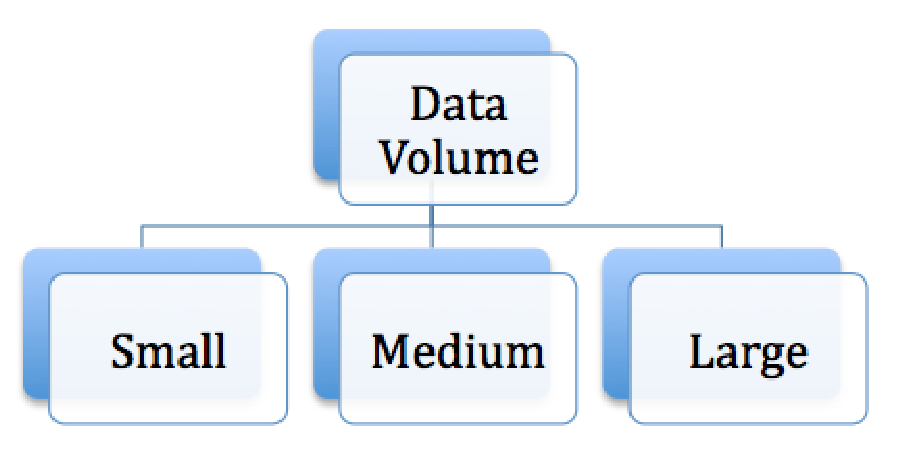
\includegraphics[scale=0.5]{../diagrams/taxonomy-data-volume}
  \caption{The Data Volume Taxonomy}
  \label{fig:taxonomy-data-volume}
\end{figure}

\begin{itemize}
  \item \textbf{Small}: sensor networks whose annual production of data is in the
  range of MBs or to 1GB of data, usually stored in flat files directly in the
  operating system. They are usually collected from sensor devices that only
  generate numerical data;
  \item \textbf{Medium}: amount of data that ranges from GBs to 1TB data and is 
  managed using disk arrays;
  \item \textbf{Large}: the amount of data produced by a sensor device ranging 
  from TBs to 1PT of data necessitates the construction of a data center 
  specializing in the storage of data produced by sensor devices, taking into 
  account the addition of data provenance, among others.
\end{itemize}

\section{System Organization Taxonomy} 

Different approaches have been developed to organize the storage of data
produced from sensor networks. Figure \ref{fig:taxonomy-database-architecture}
describes the taxonomy of the database system organization as follows:

\begin{figure}[h]
  \centering
  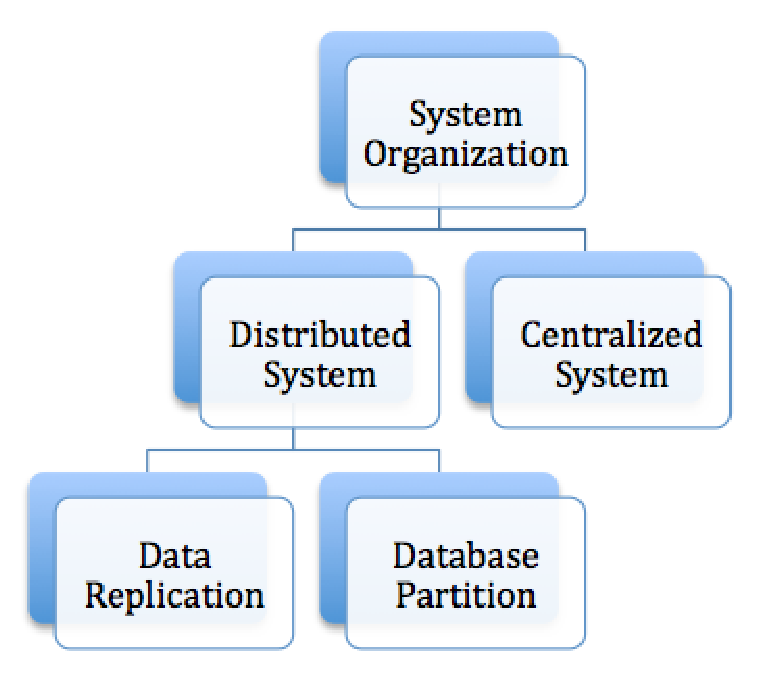
\includegraphics[scale=0.5]{../diagrams/taxonomy-database-architecture}
  \caption{The System Organization Taxonomy}
  \label{fig:taxonomy-database-architecture}
\end{figure}

\begin{itemize}
  \item \textbf{Centralized System}: a database system that runs in one single
  centralized host, the focus being the managing of the collected data
  \cite{sn-intro01}. When the system is organized in a centralized system,
  usually a centralized query processing is used to process any request to
  operations on the database management system;
  \item \textbf{Distributed System}: a database system that can be composed of
  more than one node. Usually, the use of the pattern of Master-Slave
  mechanism or data replication \cite{sn-data-center-replication-load-balance} 
  is used to alleviate ``hot spots'' during concurrent processes of data
  collection from the sensor devices and data access from the final users.
  Unique mechanisms can be used to disaggregate the produced data from a
  concentrated one: the use of database partitioning, as related to the
  data-centric storage, where each partition is responsible to handle data
 produced by a given type of sensor, for instance. Finally, it is the type of
 system used to support in-network query processing.
\end{itemize}

\section{Relationships among the Taxonomies}

On the whole, the taxonomies described in this chapter were based solely on the
literature review described in the previous chapter. They can be helpful in 
understanding the requirements of a data persistence layer for sensor networks
with different infrastructures. They are summarized on Table 3.1, and briefly
highlight these relationships in order to better analyze a problem related to data persistence.

\begin{table}[!b]
    \label{tab:taxonomies-list-summary}
    \begin{center}
        \begin{tabular}{|p{170pt}|p{250pt}|}\hline 
        \textbf{Taxonomy Name} & \textbf{Associated Taxas}\\\hline 
        Purpose of the Sensor Data & Real-time Data Stream, Data Archival \\\hline 
        Location of the Sensor Data & Local Storage, External Storage\\\hline
        Data Model & Schema-Dependent, Schema-less Models\\\hline 
        Data Description & Provenance-Aware, Annotations\\\hline
        Query Processing & In-Network Query, Centralized Query\\\hline 
        Data Volume & Small, Medium, Large\\\hline
        System Organization & Centralized System, Distributed System\\\hline
        \end{tabular}
    \end{center}
    \caption{Summary of the Data Persistence Taxonomies}
\end{table}

The taxonomy related to the purpose of the sensor data can be directly associated 
with the taxonomy of the location of the sensor data. While the taxon of the 
real-time data stream relates to the local data storage, the taxon related to
data archival correlates the storage of the collected data with an external
storage one. In addition to that, the converse is also true.

The taxonomy related to the data model can be linked to any taxon from the 
system organization because it is used in both centralized and distributed
systems, also associated with the location of the data and, consequently, the
query processing method used. Furthermore, the data description taxon can be
used by any of the data models. 

The query processing is directly related to the location of the collected data
and with the system organization taxa. While centralized systems use centralized
query processing methods, in-network query processing is when the collected
data is located in different external storage devices organized in a
data-centric way, usually supported by a distributed system.

Similarly, the taxonomy related to the volume of data produced by a sensor
network usually determines the system organization used to handle and process
the collected data. When the volume is small, the use of a single server is
required, usually using an external storage device, which relates to the
taxonomy for storage systems. However, when the volume is medium to large, the
use of distributed systems is required to cope with high volume of data
processing. Techniques described for data replication is used to decrease the
load in hot spots of the architecture. On the other hand, approaches to
separate the data being written and read can be used such as Load Balancing or
Database Partition, and the use of a Data-Centric storage approach is used.

In the light of these taxonomies, the classification of the data persistence
properties of a sensor networks can be studied and reviewed. As described in
the introduction of this report, one the main motivations for this work
was to provide means of data persistence for NetBEAMS, a case study which does
not contain a data layer. Therefore, the following chapter seeks to describe
NetBEAMS and its supporting infrastructure.
